\documentclass{standalone}

\usepackage{tikz}
\begin{document}

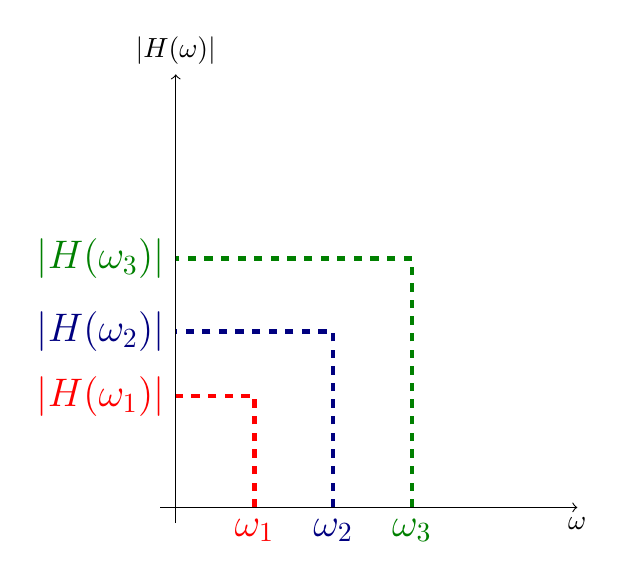
\begin{tikzpicture}[domain = 0:5, samples = 1000]
  \draw[->] (-0.2,0) -- (5.1,0) node[below] {$\omega$};
  \draw[->] (0,-0.2) -- (0,5.5) node[above] {$|H(\omega)|$};

  \draw[dashed,-,ultra thick,color=red] (1,0) node[font = \Large, below] {$\omega_1$} -- (1,1.4142) -- (0,1.4142) node[font = \Large, left] {$|H(\omega_1)|$};
  \draw[dashed,-, ultra thick,color =blue!50!black] (2,0) node[font = \Large, below] {$\omega_2$} -- (2,2.236) -- (0,2.236) node[font = \Large, left] {$|H(\omega_2)|$};
  \draw[dashed,-,ultra thick,color=green!50!black] (3,0) node[font = \Large, below] {$\omega_3$} -- (3,3.1622) -- (0,3.1622) node[font = \Large, left] {$|H(\omega_3)|$};

 \draw[ultra thick, color=black] plot[id=cero] function{sqrt(1+x**2)};

\end{tikzpicture}

\end{document}
